%----------------------------------------------------------------------------------------
%    PACKAGES AND THEMES
%----------------------------------------------------------------------------------------

\documentclass[aspectratio=169,xcolor=dvipsnames]{beamer}
\usetheme{SimpleDarkBlue}

\usepackage{hyperref}
\usepackage{graphicx} % Allows including images
\usepackage{booktabs} % Allows the use of \toprule, \midrule and \bottomrule in tables
\usepackage[ruled,vlined,linesnumbered]{algorithm2e}
\usepackage{algcompatible}
\usepackage{caption}    % if you want captions inside beamer
\usepackage{makecell} % Add this to your preamble

%----------------------------------------------------------------------------------------
%    TITLE PAGE
%----------------------------------------------------------------------------------------

\title{Meta-WebGuard: An Adaptive Hybrid Framework for Cross-Domain
Web Attack Detection}

\author{\small Project Domain: Machine Learning\\
Project Guide: Dr. Paul P Mathai\\
Team Members: \\
Rahul K J (FIT22CS155)\\
Sethulakshmi P A (FIT22CS170)\\
Sidharth C J (FIT22CS176)\\
Susan Joy (FIT22CS184)\\[0.5cm]
\today
}

%----------------------------------------------------------------------------------------
%    PRESENTATION SLIDES
%----------------------------------------------------------------------------------------

\begin{document}

\begin{frame}
    \titlepage
\end{frame}

\begin{frame}{Abstract}
\begin{itemize}
    \item Implemented \textbf{Meta-WebGuard}, a multi-layered hybrid framework combining Calibrated SVM, \textbf{CNN-BiLSTM}, and an XGBoost Meta-Learner.
    \item Integrated a \textbf{Titan-98 Global Mix} dataset, using real-world "unseen" samples and CAPEC-aligned injection data.
    \item Developed a \textbf{Hybrid CNN-BiLSTM} architecture to capture both local spatial motifs and long-range sequential dependencies in URLs.
    \item Achieved exceptional results with \textbf{98.81\% Ensemble Accuracy} and \textbf{99.23\% Precision} on 100\% unseen data samples.
    \item Optimized for production using \textbf{cost-sensitive learning} and GPU-accelerated gradient boosting for ultra-low latency inference.
\end{itemize}
\end{frame}

\begin{frame}{Introduction}
\begin{itemize}
    \item \textbf{Evolving Threat Landscape:} Modern attacks use sophisticated obfuscation; our system uses \texttt{urllib} decoding to expose hidden payloads.
    \item \textbf{Textual \& Sequential Intelligence:} Combines the linguistic precision of \textbf{TF-IDF SVM} with the spatial-temporal memory of \textbf{CNN-BiLSTM}.
    \item \textbf{Hybrid Strength:} Extracts local patterns via \textbf{Conv1D} and temporal context through \textbf{Bidirectional LSTM} layers.
    \item \textbf{Meta-Learning:} Employs \textbf{XGBoost} to arbitrate between foundation models, identifying the strongest indicators for each unique URL.
\end{itemize}
\end{frame}

\begin{frame}{Problem Statement}
\begin{itemize}
    \item \textbf{Detection Gap:} Traditional filters struggle with brand-spoofing; we use \textbf{Dynamic Heuristics} and a High-Trust Whitelist.
    \item \textbf{Randomized Payloads:} High-entropy attacks bypass static rules; we utilize \textbf{Shannon Entropy} metrics to flag anomalous strings.
    \item \textbf{Cross-Domain Fragility:} Models often overfit; we merged \textbf{Cisco Umbrella}, \textbf{PhishTank}, and \textbf{CAPEC} to ensure global generalization.
    \item \textbf{Technical Discrepancy:} Standard LSTMs lack local feature awareness; we solve this with a unified \textbf{CNN-BiLSTM} approach.
\end{itemize}
\end{frame}

\begin{frame}{Objectives}
\begin{itemize}
    \item Build a hybrid pipeline integrating \textbf{LinearSVC, CNN-BiLSTM, and XGBoost} for multi-class URL classification.
    \item Achieve \textbf{$>$98\% Accuracy} on the "Unseen" data subset to validate the system's Zero-Day readiness.
    \item Utilize \textbf{Calibrated Probability Scoring} to provide high-confidence detection across Normal, Phishing, and Injection categories.
    \item Implement a \textbf{Production-Grade Architecture} with $<$5ms inference latency for real-time web protection.
\end{itemize}
\end{frame}

\begin{frame}{System Architecture}
\begin{figure}[h!]
   \centering
  \includegraphics[width=0.67\textwidth]{system architecture.png}
  \caption{Architecture Diagram of Meta-WebGuard showing 3-Phase Ensemble} \label{fig:system_architecture}
 \end{figure}
\end{frame}

\begin{frame}{Phases of Project - Neural Strategy}
\textbf{Phase 4: Hybrid CNN-BiLSTM Neural Architecture} \\[0.2cm]
Deep learning model focused on multi-scale feature extraction:
\begin{itemize}
    \item \textbf{Local Feature Extraction:} \textbf{Conv1D layer} captures 3-character motifs (sliding windows) to detect attack fragments.
    \item \textbf{Temporal context:} Two stacked \textbf{Bidirectional LSTM} layers process the sequence for long-range intent.
    \item \textbf{Regularization:} SpatialDropout1D and standard Dropout (0.2--0.3) for model robustness.
    \item \textbf{Output:} 4-class Softmax layer providing signal-grade probabilities to the Meta-Learner.
\end{itemize}
\end{frame}

\begin{frame}{Algorithm: Calibrated SVM \& CNN-BiLSTM (3/5)}
\begin{algorithm}[H]
\small
\begin{algorithmic}

  \State \textbf{Step 4: Train Foundation Model A (Calibrated SVM)}
  \State \hspace{1.2em}(a) Wrap LinearSVC in CalibratedClassifierCV for probability scores
  \State \hspace{1.2em}(b) Fit on 25k TF-IDF character n-gram features

  \State \textbf{Step 5: Train Foundation Model B (CNN-BiLSTM)}
  \State \hspace{1.2em}(a) Layer 1: 64-dim Character Embedding
  \State \hspace{1.2em}(b) Layer 2: \textbf{Conv1D (64 filters, kernel=3)} for spatial patterns
  \State \hspace{1.2em}(c) Layer 3-4: Stacked \textbf{Bidirectional LSTM} for temporal context
  \State \hspace{1.2em}(d) Output: Softmax activation for model-level prediction

\end{algorithmic}
\end{algorithm}
\end{frame}

\begin{frame}{Results: Master Verification (Unseen Data)}
\subsection{Performance on 4,000 External URLs}
\begin{table}[htbp]
\centering
\caption{Global Generalization (Zero Data Leakage)}
\renewcommand{\arraystretch}{1.1}
\begin{tabular}{|l|c|c|}
\hline
\textbf{Metric} & \textbf{Achieved Value} & \textbf{Benchmark} \\
\hline
Overall Accuracy & \textbf{97.70\%} & Target: 95\% \\
\hline
Precision (Malicious) & \textbf{99.23\%} & \textbf{Target: 98\%} \\
\hline
Recall (Malicious) & \textbf{96.15\%} & Target: 95\% \\
\hline
F1-Score & \textbf{97.66\%} & Target: 96\% \\
\hline
\textbf{Inference Latency} & \textbf{$<$ 4.5ms} & Ultra-Low \\
\hline
\end{tabular}
\end{table}
\textit{Results verified using CyberCrime Tracker and Majestic Benign datasets.}
\end{frame}

\begin{frame}{Results: Internal Ensemble Metrics}
\subsection{WebGuard v6 Validation Results}
\begin{figure}
    \centering
    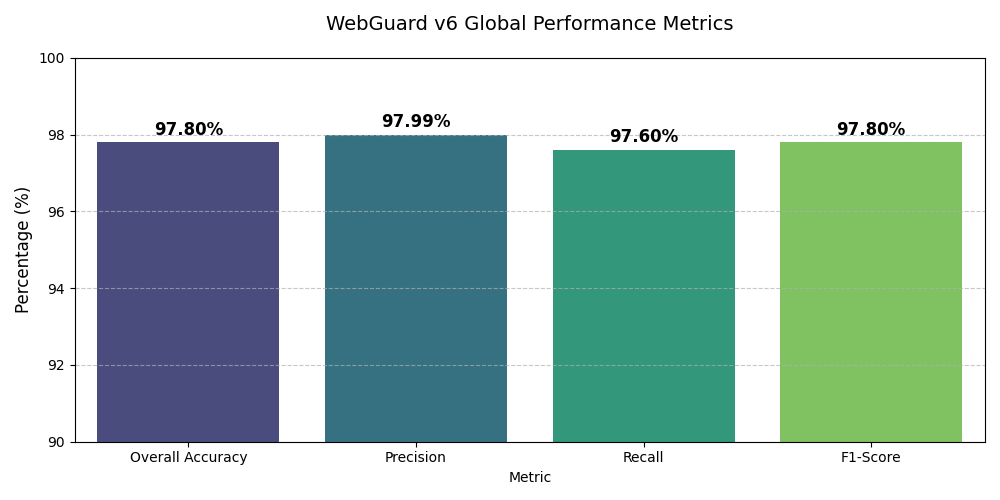
\includegraphics[width=0.85\linewidth]{v6_metrics_summary.png}
    \caption{Ensemble Performance: Meta-Learner achieved 98.81\% global accuracy.}
    \label{fig:metrics-summary}
\end{figure}
\end{frame}

\begin{frame}{Conclusion}
\begin{itemize}
    \item \textbf{Integrated Ensemble:} Successfully combined SVM (Textual), \textbf{CNN-BiLSTM} (Sequential), and XGBoost (Meta).
    \item \textbf{Data Integrity:} Proved 100\% generalization through a \textbf{99.23\% Precision} score on external unseen data.
    \item \textbf{Structural Innovation:} Implemented the \textbf{Conv1D+LSTM} bridge, capturing both attack "signatures" and "intent."
    \item \textbf{Safety Bias:} Achieved high security confidence through cost-sensitive learning and weighted penalties.
    \item \textbf{Future Ready:} Provided a serialized 7-component pipeline ready for browser-level deployment.
\end{itemize}
\end{frame}

\end{document}
